\chapter{Introducci\'on}
\label{ch:intro}

La f\'isica de astropart\'iculas experimenta actualmente un desarrollo muy veloz. 
El mensajero tradicional del cielo, el foton, ha sido complementado a principios del siglo XX con la observaci\'on de part\'iculas cargadas (rayos c\'osmicos) y, durante las \'ultimas d\'ecadas, mediante el desarrollo de la astrof\'isica de neutrinos.
Todos estos mensajeros, ricos en informaci\'on, nos permiten estudiar las propiedades de fuentes astrof\'isicas en todo el cosmos.

La astronom\'ia de neutrinos se encuentra en sus comienzos. 
Esta admite una nueva mirada al universo expandiendo las posibilidades de observaci\'on.
Los rayos c\'osmicos cargados son deflectados debido a los campos magn\'eticos intergal\'acticos mientras que los rayos gamma son absorbidos en zonas opacas del espacio. 
Sin embargo los neutrinos no sufren ninguna de estas alteraciones ya que no poseen carga el\'ectrica y adem\'as s\'olo interact\'uan mediante fuerza d\'ebil y su secci\'on efic\'az es baja.
Sin embargo, esta cualidad los hace extremadamente dif\'iciles de detectar en al tierra, lo que representa un desaf\'io muy interesante de abordar.
Existe una gran cantidad de rese\~nas sobre el estado del \'area, como por ejemplo \cite{XXX}, en las que se remarca el potencial de utilizar el neutrino como mensajero c\'osmico.

En este trabajo se aborda la detecci\'on de neutrinos c\'osmicos ultra energ\'eticos mediante detectores de superficie.
En la primer parte de esta tesis se presenta la medici\'on del flujo de neutrinos c\'osmicos en el rango energ\'etico de \cant{10^{17}}{eV} y \cant{10^{20}}{eV} con el detector de superficie del Observatorio Pierre Auger.
El cap\'itulo \ref{ch:easAuger} contiene una introducci\'on a la f\'isica de las lluvias atmosf\'ericas extendidas que generan los rayos c\'osmicos ultra energ\'eticos. 
En el cap\'itulo \ref{ch:detectorAuger} se realiza un recuento de las caracter\'isticas m\'as importantes del detector de superficie del Observatorio Pierre Auger.
M\'as adelante, en el ca\'itulo \ref{ch:estrategiaAuger} se detalla la estrategia utilizada en el experimento para medir el flujo de neutrinos c\'osmicos ultra energ\'eticos.
El proceso de simulaci\'on de la se\~nal esperada sobre el detector se aborda en el cap\'itulo \ref{ch:simulacionAuger}, mientras que la reconstrucci\~non y selecci\'on de los eventos iniciados por neutrinos se trata en el cap\'itulo \ref{ch:seleccionauger}.
Por \'ultimo en el cap\'itulo \ref{ch:resAuger} se trata el c\'alculo de la exposici\'on del observatorio al flujo, la b\'usqueda de candidatos y la comparaci\'on de los resultados con las predicciones te\'oricas.
Por otro lado, en la seunda parte de la tesis se estudia el desempe\~no que podr\'ia alcanzar un detector de superficie conformado por 90000 antenas de radio al medir el mismo flujo de neutrinos.
En el cap\'itulo \ref{ch:motivacionRadio} se exponen brevemente los motivos por los que vale la pena el estudio de este tipo de detectores.
El cap\'itulo \ref{ch:easRadio}, como complemento al cap\'itulo \ref{ch:easAuger} se estudia la emisi\'on de ondas de radio de lluvias atmosf\'ericas extendidas.
Los m\'etodos empleados en la simulaci\'on de la se\~nal sobre el detector se detalla en el cap\'itulo \ref{ch:simulacionRadio} y su caracterizaci\'on en el cap\'itulo \ref{ch:caracterizacionRadio}.
Por \'ultimo, en el cap\'itulo \ref{ch:resultadosRadio} se aborda tanto la factibilidad de la detecci\'on como el c\'alculo de la exposici\'on en un arreglo de antenas de radio.

\section{Importancia de la detecci\'on de neutrinos c\'osmicos}
%
%
%%
%%%
% 	VER EL PROPOSAL DE GRAND!
%%%
%%
%
%
El estudio de rayos c\'osmicos ultra energ\'eticos (UHECRs por sus siglas en ingl\'es) ha estimulado en gran medida la actividad experimental y te\'orica en el campo de la astrof\'isica.
Aunque su espectro de energ\'ia ha sido caracterizado en un rango sorprendente, que abarca 14 \'ordenes de magnitud, quedan muchos misterios por resolver, entre ellos su origen y sus mecanismos de aceleraci\'on.
En esta direcci\'on, la medici\'on de UHECRs cargados presenta dos grandes limitaciones, su deflexi\'on en los campos magn\'eticos y lo que se conoce como el corte GZK.
A energ\'ias por debajo de los \cant{10^{19.5}}{eV} las trayectorias desde la fuente se ven modificadas debido a la interacci\'on con los campos magn\'eticos gal\'acticos e intergal\'acticos lo que implica que la direcci\'on de arribo de los rayos a la tierra no apunta a la fuente.
Por otro lado, el corte GZK refiere al mecanismo propuesto por Greisen, Zatsepin y Kusmin~\cite{cite:Greisen,cite:Zatsepin}, que provoca una caida en el flujo de UHECRs por encima de \cant{5\times10^{19}}{eV} debido a la p\'erdida de energ\'ia inducida por la interacci\'on con el fondo c\'osmico de microondas (CMB por sus siglas en ingl\'es), via la siguiente reacci\'on:
%
\begin{eqnarray}
p + \gamma_{\rm CMB} &\rightarrow& \Delta^{+}(1232)  \rightarrow p +\pi^{0}\quad {\rm or}\quad n +\pi^{+}
\end{eqnarray}
%
La longitud de atenuaci\'on para este proceso es $L_{att}=\frac{L_{int}}{y}$, donde $y$ es la fracci\'on de energ\'ia perdida por longitud de interacci\'on y $L_{int}$ es la longitud de interacci\'on, dada por $L_{int}=(\sigma_{p\gamma}\times n_{\gamma})^{-1}$.
Valores t\'ipicos son $\sigma_{p\gamma}\sim 10^{-28}$~cm$^{2}$, $ n_{\gamma}=410\,{\rm cm}^{-3}$ and $y\sim0.5$\footnote{$y\sim0.2$ a la energ\'ia de corte y se incrementa hasta 0.5.}, resultando en 
% \begin{equation}
$L_{att}=(\sigma_{p\gamma}\times n_{\gamma}\times y)^{-1}\sim 15\mbox{ }{\rm Mpc}$. 
Ya que a estas energ\'ias los rayos c\'osmicos son mayormente extra gal\'acticos, el corte GZK limita la m\'axima energ\'ia que puede ser observada en la tierra y provocando una supresi\'on del flujo por encima de los \cant{50}{EeV}.
En la figura \ref{fig:protProp} se muestra la longitud $L_{att}$ como funci\'on de la energ\'ia para protones y n\'ucleos de hierro. 
Es posible observar como a partir de los \cant{50}{EeV} esta cantidad decae hasta un tama\~no inferior al del Super cluster de Virgo a los \cant{1000}{EeV}.
%
\begin{figure}[ht]
	\begin{center}
	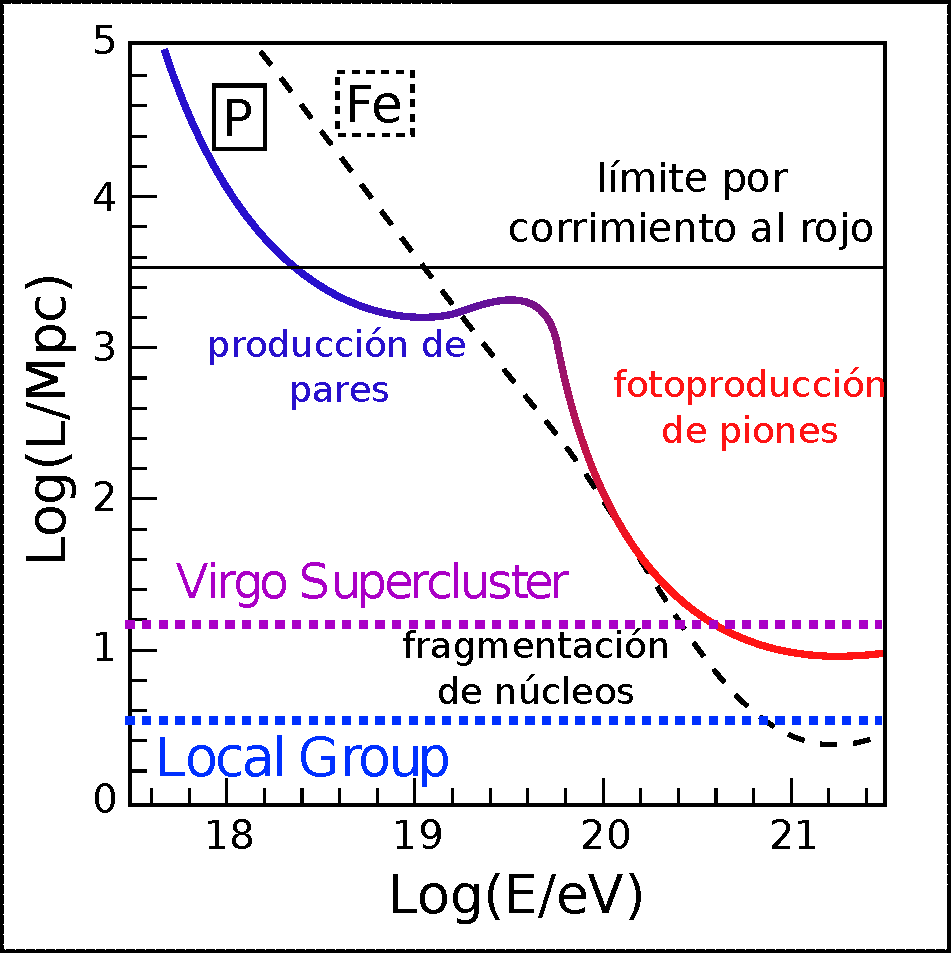
\includegraphics[width=0.55\textwidth]{fig/introduccion/proton_propaga_espanol}
	\caption{\label{fig:protProp} Longitud de atenuaci\'on como funci\'on de la energ\'ia para protones y n\'ucleos de hierro. Se observa que a partir de \cant{50}{EeV} esta cantidad decae hasta el tama\~no del Super cluster de Virgo a los \cant{1000}{EeV}.}
	\end{center}
\end{figure}
%

Por otro lado, el observatorio Pierre Auger ha medido el flujo de rayos c\'osmicos combinando un detector de superficie con t\'ecnicas de fluorescencia y ha acumular suficiente estad\'istica para medir el flujo con presici\'on hasta alrededor de \cant{2\times10^{20}}{eV}. 
Tambi\'en pudo corroborar la supresi\'on del flujo para energ\'ias superiores a los \cant{10^{19.6}}{eV}~\cite{cite:AugerSpectrum}, tal como se observa en la figura \ref{fig:specGZK}.
%
\begin{figure}[ht]
	\begin{center}
	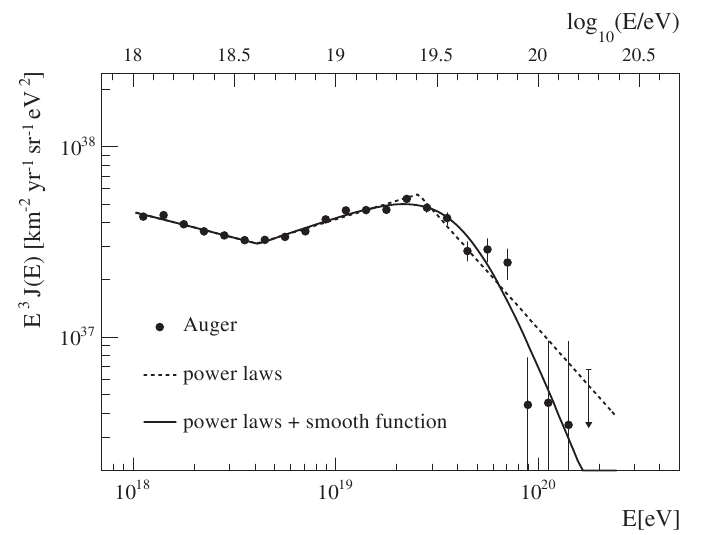
\includegraphics[width=\textwidth]{fig/introduccion/spectrum_withGZK}
	\caption{\label{fig:specGZK} Espectro de UHECRs medido con el observatorio Pierre Auger. En l\'inea punteada se muestra el ajuste por leyes de potencia partidas y en l\'inea llena la dos leyes de potencia y una funci\'on suave. Las barras corresponden al error estad\'istico de cada punto, mientras que el error sistem\'atico representa el $22\%$ de la energ\'ia.}
	\end{center}
\end{figure}

De manera similar, el flujo de fotones ultra energ\'eticos, por encima de \cant{\sim 10^{14}}{eV}, no puede ser de naturaleza extra gal\'actica, debido a la producci\'on de pares en la interacci\'on con fotones del fondo de microondas, seg\'un\cite{cite:photonInt1,cite:photonInt2}:
%
\begin{equation}
\gamma_{UHE} + \gamma_{CMB} \rightarrow e^- + e^+
\end{equation}
%
En la figura \ref{fig:photProp} se grfica la longitud de atenuaci\'on de los fotones como funci\'on de la energ\'ia\footnote{En este caso, la longitud de atenuaci\'on corresponde con la distancia necesaria para que el flujo se reduca a la mitad.}
%
\begin{figure}[ht]
	\begin{center}
	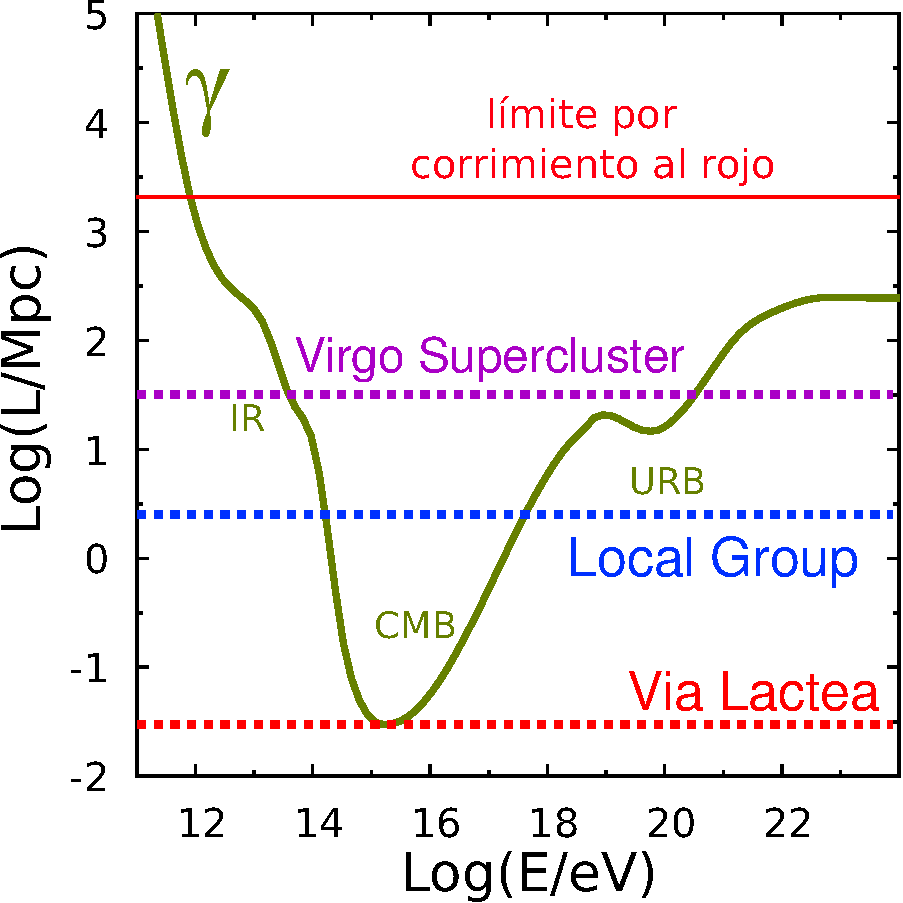
\includegraphics[width=0.55\textwidth]{fig/introduccion/photon_propaga_espanol}
	\caption{\label{fig:photProp} Longitud de atenuaci\'on para fotones. Los $\gamma$ con energ\'ias entre \cant{10^{14}}{eV} y \cant{10^{18}}{eV} pr\'acticamente no pueden alcanzar la tierra desde distancias mayores a \cant{1}{Mpc}. Las etiquetas IR, CMB y URB (ver texto) corresponden al fondo dominante contra el que interact\'uan los $\gamma_{UHE}$.}
	\end{center}
\end{figure}
%
Dependiendo de la energ\'ia, los $\gamma_{UHE}$ pueden interactuar tambi\'en con el fondo de radiaci\'on infraroja (IR)\cite{cite:IR} y con el fondo de radio universal (URB)\cite{cite:URB}.

Como consecuencia el tercer mensajero $-$ el neutrino $-$ cobra una importancia adicional, lo que convirti\'o su detecci\'on en uno de los mayores logros de la astrof\'isica contempor\'anea.
Esto se debe a que los neutrinos no sufren ninguna de las desventajas mensionadas hasta el momento. 
Debido a que interact\'uan mediante interacci\'on d\'ebil y a que su secci\'on efic\'az resulta extremadamente peque\~na, pueden viajar distancias cosmol\'ogicas e incluso escapar de la regi\'on en la que fueron producidos casi sin p\'erdidas de energ\'ia.
Por otro lado, debido a que son el\'ectricamente neutros su trayectoria no se ver\'a deflectada debido a la interacci\'on con los campos magn\'eticos intra y extra gal\'acticos.
Por este motivo, la direcci\'on de arribo de los neutrinos c\'osmicos detectados guardar\'a completamente la informaci\'on del lugar del universo en el que fueron producidos.
Por estos motivos, los neutrinos representan una opci\'on \'unica, que permite detectar directamente posibles fuentes de UHECRs.

En las siguientes secciones de este cap\'itulo se presentar\'a una discusi\'on sobre las posibles fuentes y flujos de neutrinos c\'osmicos ultra energ\'eticos, a saber, el mecanismo GZK, n\'ucleos de galaxias activos (AGN) y explosiones de rayos gamma (GRB).
Tambi\'en se realizar\'a un recuento de los ezfuersos experimentales pasados, presentes y futuros en este campo.

\section{Posibles fuentes y flujos esperados}

Existen varios modelos en la literatura que predicen flujos de neutrinos c\'osmicos ultra energ\'eticos.
La la supresi\'on observada en el flujo por encima de los \cant{50}{EeV} refuerza la idea de la existencia de un flujo difuso de neutrinos cosmog\'enicos.
En este caso, estos son producidos durante la propagaci\'on de un UHECR a trav\'es del universo. 
Adem\'as pueden ser producidos en la aceleraci\'on de protones y nucleos en n\'ucleos de galaxias activos (o AGN por sus siglas en ingl\'es)\cite{cite:nuAGN} o por producci\'on de fotopiones en explosiones de rayos gamma (GRB por sus siglas en ingles)\cite{cite:nuGRB}.
Detectores como AMANDA o IceCube, su sucesor, se encuentran bien posicionados para realizar b\'usquedas de fuentes con espectros de ley de potencia fuertes ($\propto E^{-2}$) en el rango que comprende desde el TeV  hasta el PeV. 
Para fuentes cuyo flujo presenta un m\'aximo en energ\'ias por encima de los \cant{100}{PeV} el flujo predicho resulta ser peque\~no, requiriendo detectores con mayor exposici\'on.

Otros posibles mecanismos de producci\'on de neutrinos c\'osmicos estan relacionados con el decaimiento de part\'iculas ex\'oticas extremadamente masivas tales como defectos topol\'ogicos\cite{cite:nuTopDefects}, o con la interacci\'on de neutrinos energ\'eticos con el fondo de neutrinos del Big-Bang via la resonancia Z-burst\cite{cite:nuZBurst_init}.
Estos flujos, que pretend\'ian explicar el origen de los rayos c\'osmicos ultra energ\'eticos, han sido fuertemente constre\~nidos por los experimentos m\'as recientes\cite{cite:nuConstraintsTD}.
En las siguientes secciones se desarrollas las ideas enumeradas hasta aqu\'i.

	\subsection{Neutrinos GZK}
	\label{sbsc:introGZK}
	Greisen, Zatsepin and Kusmin propusieron que los rayos c\'osmicos cuya energ\'ia supere los \cant{5\times10^{19}}{eV}, al propagarse por el universo interactuar\'an con el fondo de microondas produciendo neutrinos, seg\'un la ecuaci\'on \ref{eq:pionDecay}.
	\begin{equation}\label{eq:pionDecay}
	\pi^{+} \rightarrow \mu^{+}+ \nu_{\mu} \rightarrow e^{+} + \nu_{e} + \bar{\nu}_{\mu} + \nu_{\mu}
	\end{equation}
	
	\begin{figure}[ht]
		\begin{center}
		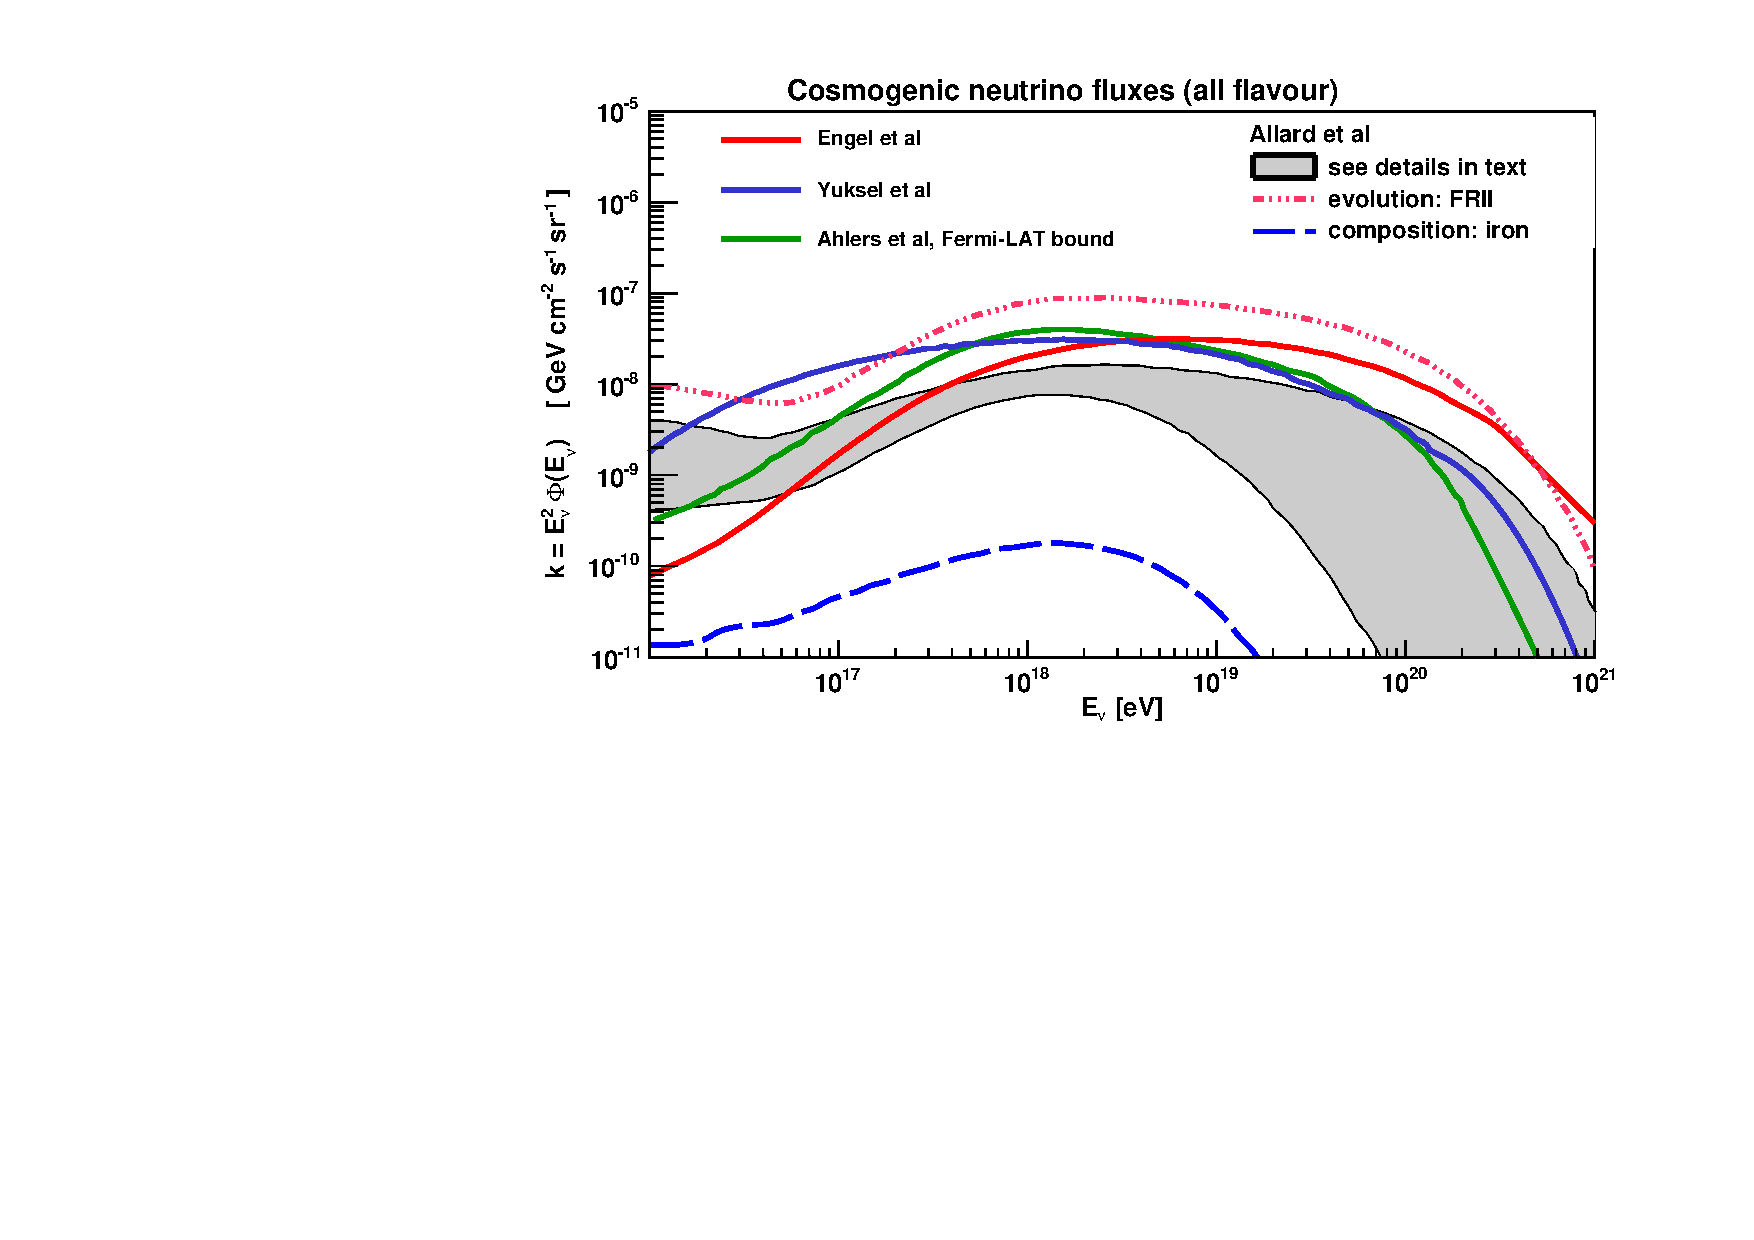
\includegraphics[width=\textwidth]{fig/introduccion/gzk_fluxes}
		\caption{\label{fig:flujosGZK} }
		\end{center}
	\end{figure}
	
	\subsection{AGNs y GRBs}
	
	\begin{figure}[ht]
		\begin{center}
		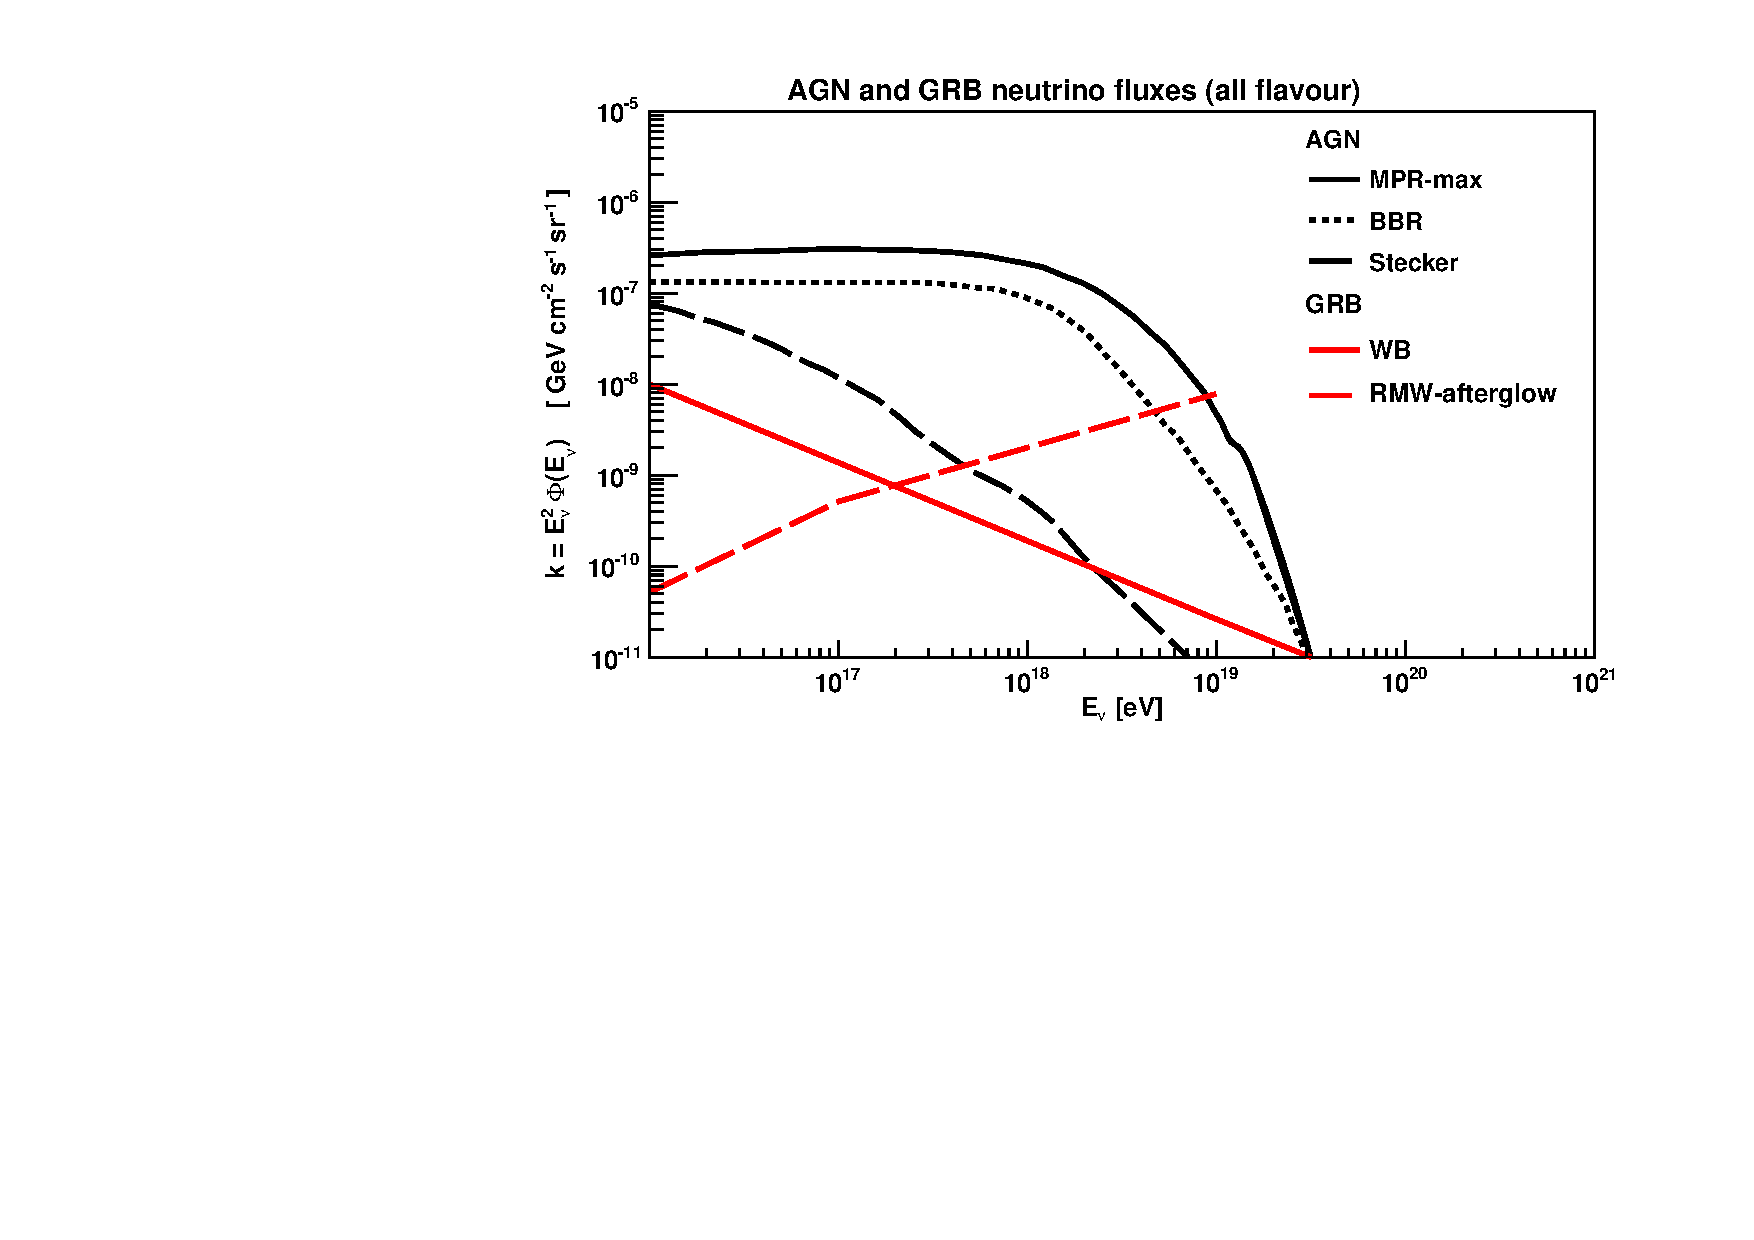
\includegraphics[width=0.75\textwidth]{fig/introduccion/AGN_GRB_nufluxes}
		\caption{\label{fig:flujosAGN} }
		\end{center}
	\end{figure}
	
	\subsection{Fuentes no convencionales}
	
	\begin{figure}[ht]
		\begin{center}
		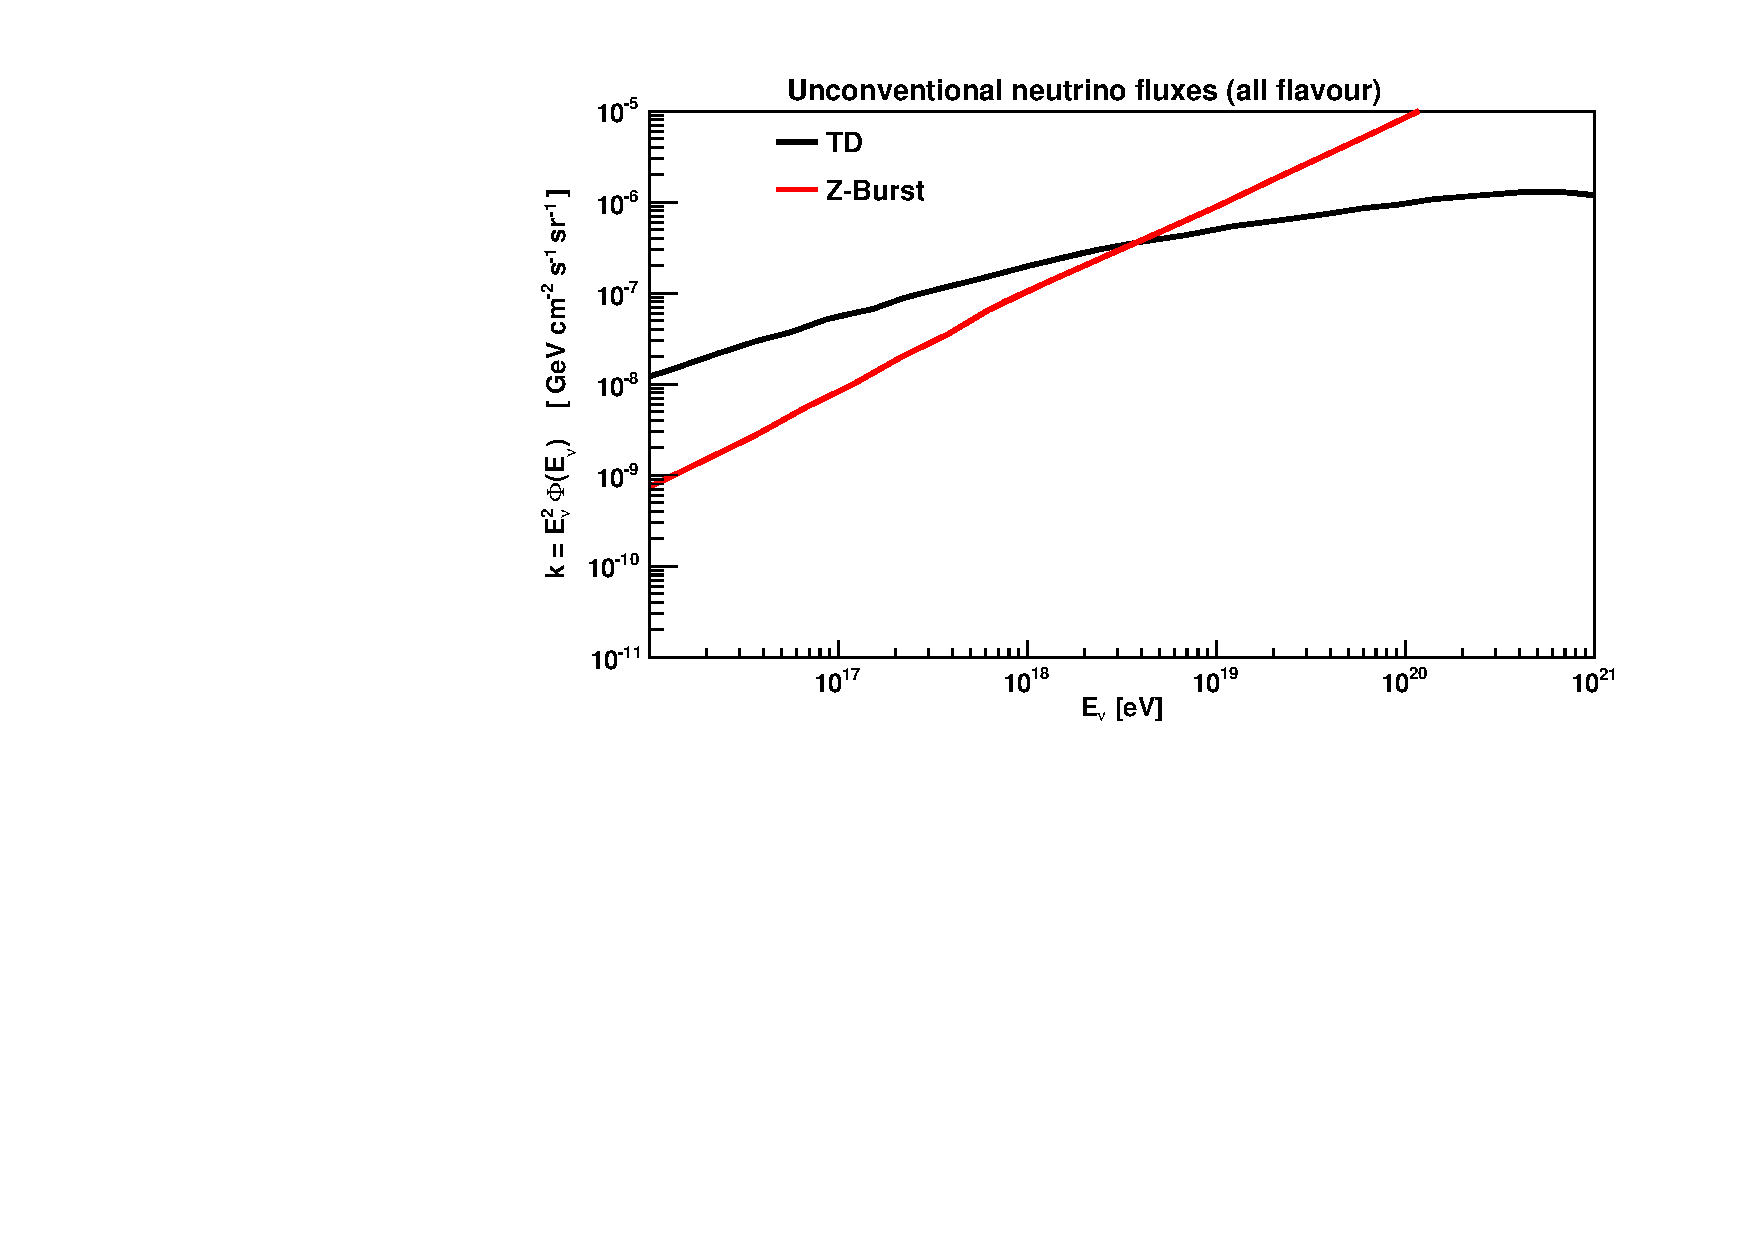
\includegraphics[width=0.75\textwidth]{fig/introduccion/unconventional_nuFluxes}
		\caption{\label{fig:flujosNoConv} }
		\end{center}
	\end{figure}

\section{Búsquedas de neutrinos cósmicos ultra energéticos}

% \section{Nacimiento de la astronom\'ia de neutrinos c\'osmicos}

